%  Doc on OneDrive: To be added by AA
%  Shared forlder with resources: to be created by AA

\documentclass[conference]{IEEEtran}
%\documentclass {article}

\usepackage[table]{xcolor} % to color inside equation
\usepackage{array}
\usepackage{caption}
\usepackage{subcaption}
\usepackage{tabularx}
\usepackage{booktabs}
\usepackage{longtable}
\usepackage{multirow}
\usepackage{colortbl}
\usepackage{hhline}
\usepackage{tabularx,colortbl}
% \usepackage{algorithmic}
\usepackage[ruled]{algorithm2e}

%%
\usepackage{amsmath,varwidth,array,ragged2e}
\usepackage[colorlinks=true]{hyperref} % to use \autoref instead of \ref
\usepackage{cleveref}
\renewcommand{\sectionautorefname}{Section}

\usepackage{cite}
\usepackage{amsmath,amssymb,amsfonts}
\usepackage{mathrsfs} % for \mathscr
% \usepackage{algorithmic}
% \usepackage{graphicx}
\usepackage{float}
% \usepackage{epsfig}
% \usepackage{epstopdf}
\usepackage{enumitem}
\usepackage{soul}

\usepackage{lipsum}

% \usepackage{subfig}
\usepackage{mathtools} % matrix alignment

\usepackage{color}
\usepackage[dvips]{graphicx}

% Acronym package (Choose one of the following options)
% \usepackage{acronym} % if you want to show the list of abbreviations
\usepackage[nolist]{acronym} % if you do not want to show the list of abbreviations
% How to use:
% \ac{id} -> 

%\usepackage{qtree}
\usepackage{tikz}
%%\usetikzlibrary{trees}
\usepackage[english]{babel}
\usepackage{authblk}

% \definecolor{seagreen}{rgb}{0.18, 0.55, 0.34} % for comments in algorithms
% \SetAlFnt{\small\color{black}\tt}
% \LinesNumbered
% \renewcommand{\DataSty}[1]{{\color{yellow}\texttt{#1}}}
% \renewcommand{\KwSty}[1]{{\color{blue}\texttt{#1}}}
% \renewcommand{\ProgSty}[1]{{\color{black}\texttt{#1}}}
% \renewcommand{\FuncSty}[1]{{\color{black}\texttt{#1}}}
% \renewcommand{\CommentSty}[1]{{\color{seagreen}\texttt{#1}}}
% \renewcommand{\ArgSty}[1]{{\color{black}\texttt{#1}}}
% \renewcommand{\FuncArgSty}[1]{{\color{black}\texttt{#1}}}
% \renewcommand{\ProcArgSty}[1]{{\color{black}\texttt{#1}}}
% \renewcommand{\ProcNameSty}[1]{{\color{black}\texttt{#1}}}
% \renewcommand{\NlSty}[1]{{\color{black}\texttt{#1}}}
% \newcommand{\red}[1]{{\textcolor{red} {#1}}}
% \newcommand{\blue}[1]{{\textcolor{blue} {#1}}}
% \definecolor{mygreen}{rgb}{0, 0.5, 0}
% \newcommand{\green}[1]{{\textcolor{mygreen} {#1}}}

% \makeatletter
% \newcommand\notsotiny{\@setfontsize\notsotiny\@vipt\@viipt}
% \makeatother

% \makeatletter
% \newcommand*\bigcdot{\mathpalette\bigcdot@{.5}}
% \newcommand*\bigcdot@[2]{\mathbin{\vcenter{\hbox{\scalebox{#2}{$\m@th#1\bullet$}}}}}
% \newcommand{\mathbold}[1]{\text{\textbf{#1}}}
% \newcommand{\mathbolditalic}[1]{\text{\textit{\textbf{#1}}}}
% \newcommand{\etal}{\textit{et al. }}
% \makeatother

% \newcommand{\figref}[1]{Figure~\ref{#1}}
% \newcommand{\algoref}[1]{Algorithm~\ref{#1}}
% \newcommand{\tableref}[1]{Table~\ref{#1}}
% \newcommand{\listref}[1]{Listing~\ref{#1}}
% \newcommand{\secref}[1]{Section~\ref{#1}}


% %\usepackage{caption,setspace} % For caption Problem
% %\captionsetup{font={small,stretch=0.80}}

% \usepackage{textcomp}
% \def\BibTeX{{\rm B\kern-.05em{\sc i\kern-.025em b}\kern-.08em
%     T\kern-.1667em\lower.7ex\hbox{E}\kern-.125emX}}


% \DeclareRobustCommand*{\IEEEauthorrefmark}[1]{%
%   \raisebox{0pt}[0pt][0pt]{\textsuperscript{\footnotesize #1}}%
% }

% \definecolor{lightgray}{gray}{0.9} % fot tables

% green highlight
\definecolor{g}{rgb}{0.56, 0.93, 0.56}
\DeclareRobustCommand{\hlg}[1]{{\sethlcolor{g}\hl{#1}}}
% blue highlight
\definecolor{bb}{rgb}{0.56, 0.86, 0.93}
\DeclareRobustCommand{\hlb}[1]{{\sethlcolor{bb}\hl{#1}}}

% % restore footnote line as it is removed in the document class file
% \makeatletter
% \def\footnoterule{\kern-3\p@
%   \hrule \@width 2in \kern 2.6\p@} % the \hrule is .4pt high
% \makeatother

% \DeclareMathAlphabet{\mathpzc}{OT1}{pzc}{m}{it}


% % Bold \ell
% \newcommand*\Bell{\ensuremath{\boldsymbol\ell}}

% Workaround for the URL alignment in the bibliography. Note that this solution does not work with the Latex compiler, so consider changing the compiler if you are using overleaf to see the effect.
\usepackage{url}
\usepackage{breakurl}
\def\UrlBreaks{\do\/\do-}

\title{Large-Scale Vehicle Trajectory Reconstruction with Camera Sensing Network Summary}
\vspace{-10mm}

\author[1]{Ahmed Bakr}

\affil[1]{Department of Computer Science, University of Alabama, AL, USA}
%\vspace{-5mm}



\begin{acronym}
    \acro{lpr}[LPR]{License Plate Recognition}
    \acro{re-id}[Re-ID]{Re-Identification}
    \acro{mds}[MDS]{Multi-Dimensional Similarity}
    \acro{gcn}[GCN]{Graph Convolution Network}
    \acro{rng}[RNG]{Road Network Graph}
    \acro{dl}[DL]{Deep Learning}
    \acro{crnn}[CRNN]{Convolutional Recurrent Neural Network}
    \acro{hris}[HRIS]{History based route inference system}
    % \acro{}[]{}
\end{acronym}

\begin{document}

\maketitle

%% Comment to hide page number
% \thispagestyle{plain}
% \pagestyle{plain}    

% \chaptermark{Abbreviation}
% \chapter*{List of Abbreviations}

\begin{abstract}
Vehicle trajectories are crucial for understanding urban mobility and benefiting various applications.
Modern vehicle sensing solutions may not fully understand all vehicle trajectories.
In this paper, we present a summary of the paper \cite{tong2021large}, where VeTrac is proposed, which uses widely deployed traffic cameras throughout the city as a sensing network to track and reconstruct vehicle trajectories on a large scale with greater accuracy than previous work.
% I might get rid of the following sentence.
A graph convolution process ensures consistency across camera observations, while a self-training process reconstructs vehicle trajectories with confidence through alignment with the urban road network.
In real-world experiments, VeTrac achieved 98\% accuracy for simple expressways and 89\% accuracy for complex urban environments using over 7 million vehicle snapshots from over 1,000 traffic cameras.
The accuracy achieved surpasses alternatives by 32\% for expressways and 59\% for complex urban environments.
\end{abstract}

\acresetall % reset acronyms


\section{Introduction}
\label{sec:introduction}
% Motivation.
Understanding the moving trajectories of millions of vehicles in a city offers valuable insights into urban mobility, enabling applications such as usage-based electronic toll collection, accurate traffic analysis, intelligent traffic light control, and retrospective urban planning analysis.
% Related work.
Current trajectory reconstruction methods rely on in-vehicle devices (e.g., GPS) for partial knowledge, and roadway monitoring with flow sensors (e.g., loop detectors, piezoelectric sensors, infrared sensors) for capturing traffic flows.

% Their work and contributions.
This research explores the use of traffic cameras as a sensing network to accurately recreate citywide vehicle trajectory.
The traffic camera network offers advantages over existing alternatives, including: (i) Traffic cameras are widely available and cost-effective for urban deployment; (ii) They provide high coverage for sensing and monitoring vehicle trajectories; (iii) Advanced image analysis techniques can extract vehicle identifiers, enabling trajectories recovery with higher accuracy.
Vetrac was experimented on using real-world data collected from one full day of one of China's urban road networks, which covers $66 km^2$.
\Cref{fig:china-road-representation} represents the road network, where white dots present rear-view cameras, while red dots present front-view cameras.
Each camera records the following information: camera metadata, snapshot, entering time, exit time, and lane directions.
Overall, seven million snapshots were collected, and 1,247,835 vehicle trajectories have been reconstructed.

\begin{figure}
\centering
  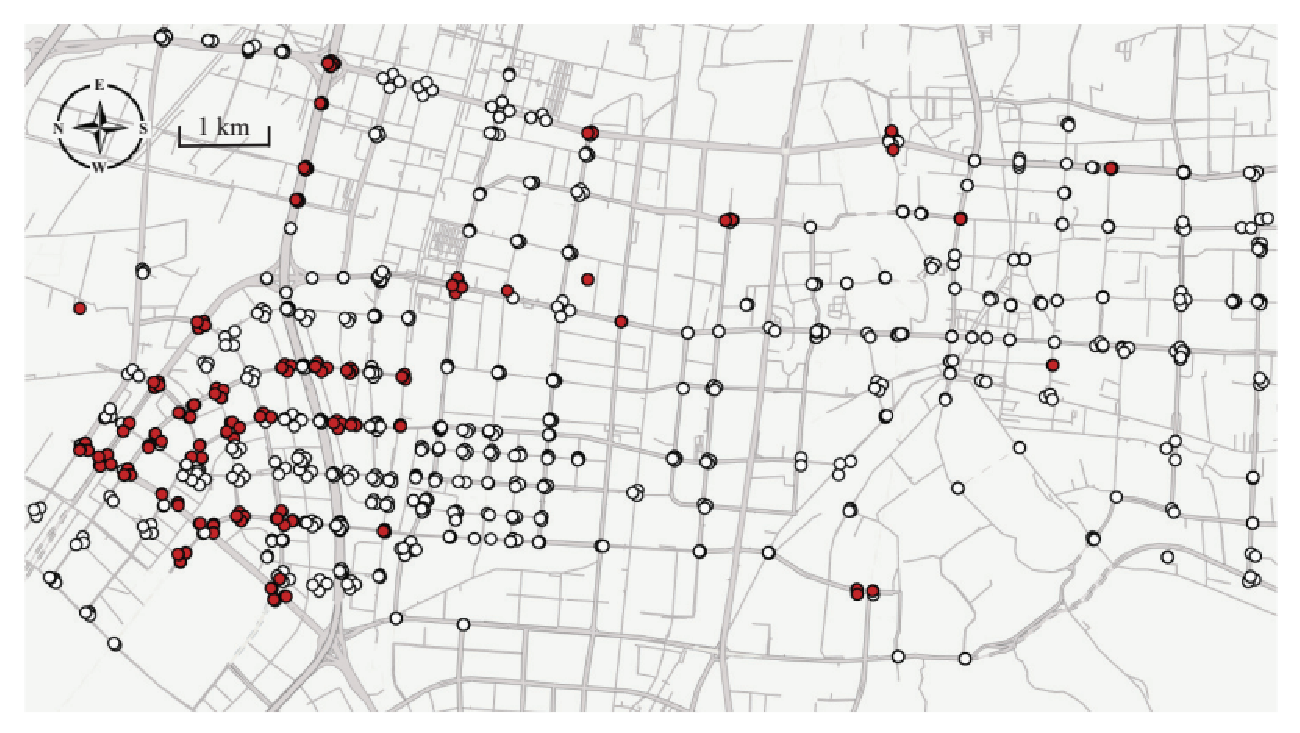
\includegraphics[width=0.9\linewidth]{figures/china-road-network.eps}
  \caption{China's road network \cite{tong2021large}}
  \label{fig:china-road-representation}
  %\vspace{-5mm}
\end{figure}

The structure of the rest of the paper is as follows:
\Cref{sec:sensing-challenges} presents the challenges that face the current sensing techniques.
In \Cref{sec:related-work}, we present the related work, while in \Cref{sec:scheme}, we present the proposed scheme.
Moreover, the evaluations are presented in \Cref{sec:discussion_evaluations}.
Finally, the work is concluded in \Cref{sec:conclusions}.

\section{Related Works} 
\label{sec:related-work}

Most of the state of the art papers focused on mobility trajectory recovery and vision based vehicle \ac{re-id}.
For mobility based trajectory recovery, the literature has focused on using Kalman filter \cite{el2005road}, Hidden Markov Model \cite{newson2009hidden} to perform map matching.
In addition, other works have focused on the usage of GPS \cite{hassanieh2012faster} and Wifi networks \cite{liu2012push, qi2017vehicle} and vehicular network, which are costly and need users' consent.
\ac{lpr} \cite{simonyan2014very} scheme depicts common practice of obtaining vehicle trajectories from camera data only using VGG-16 network.
In \cite{liu2017provid}, vehicle \ac{re-id} scheme is presented that depends only on the visual appearance of the vehicle.
Finally, \ac{hris} scheme is presented in \cite{zheng2012reducing} that is considered as mobility-based method that reduces uncertainties of low-sampling-rate trajectories instead of looking at camera images.

\section{Proposed Scheme}
\label{sec:scheme}
\Cref{fig:vetrac-architecture} shows the overall architecture of the proposed system.
First to gain extra confidence on the vehicle identification this paper presents a new block called \ac{mds} that compares between two input images and outputs their similarity percentage.
Secondly, the similar images are grouped together by modeling complext correlations among the identified snapshots with a graph structure using \ac{gcn}.
This can be considered as snapshots classification step to achieve global optimality in assigning different snapshots based on the vehicle identities.
Thirdly, for each cluster identified in the previous step, the snapshots related to one vehicle are given to a \ac{rng}, which reconstructs the trajectory for each vehicle after removing the false positives.
This can be achieved by applying reasoning \ac{dl} techniques, such as the distances and the timestamps of the screenshots.
Most of the false positives are eliminated after identifying if it is possible for a vehicle to drive from point A (first screenshot) to point B (second screenshot) within the specified time-frame (difference between timestamps between both snapshots).
Finally, the trajectory of the vehicle is identified by sorting the timestamps of the remaining images in that cluster after removing all the false positives.

\begin{figure}
\centering
  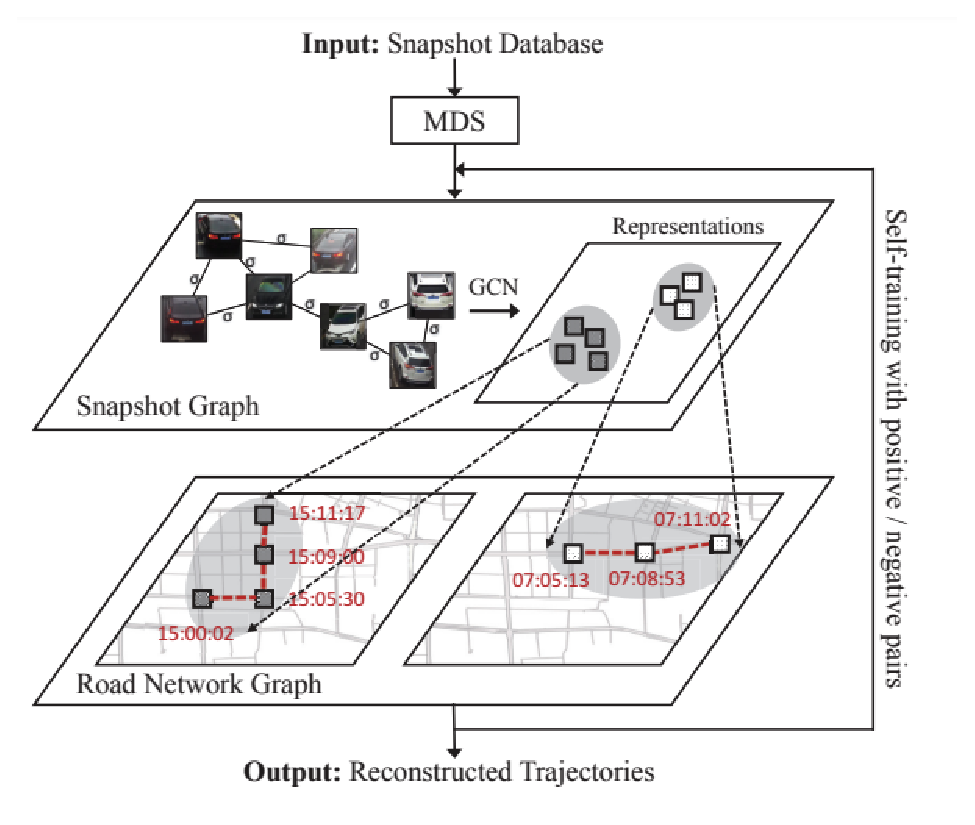
\includegraphics[width=1\linewidth]{figures/VeTrack-architecture.eps}
  \caption{VeTrac architecture \cite{tong2021large}}
  \label{fig:vetrac-architecture}
  %\vspace{-5mm}
\end{figure}

One of the main contributions of this paper is the \ac{mds} block to compare between two snapshots from two cameras in the road network.
The architecture of the block is depicted in \Cref{fig:mds-architecture} and it consists of the following three components.
\ac{lpr} similarity, appearance similarity, and mobility similarity.
Finally, the similarities of the three components are combined together as follows:
$\sigma_{A,B} = P_{plate}(A,B) * P_{app}(A,B) * P_{mob}(A,B)$, where $P_{plate}(A,B)$ is the probability that the two plates in the two snapshots A and B are similar using \ac{crnn}, while $P_{app}(A,B)$ is the probability that the appearance of the vehicle in the two snapshots are similar using the ResNet images model.
Lastly, $P_{mob}(A,B)$ is the mobility probability using an inversed Gaussian model.

\ac{lpr} uses VGGNet \cite{simonyan2014very}.
In addition, the appearance similarity block has three heads to identify the similarity of the appearance in the two snapshots.
The first head identifies the color of the vehicle.
The second head identifies the type of the vehicle, such as sedan, SUV, bus, etc.
Finally, the last head identifies the make of the vehicle, such as Audi, Honda, Nissan, etc.
The mobility head compares the time stamps of the two snapshots and given the knowledge of the road network, it outputs a probability that a car can drive from the point where the first snapshot was taken to the point where the second snapshot was taken.


\begin{figure}
\centering
  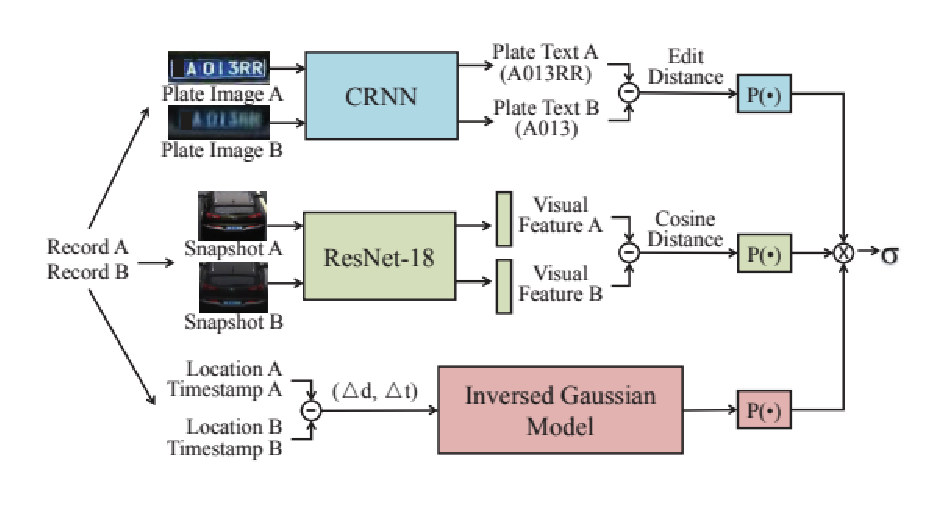
\includegraphics[width=0.9\linewidth]{figures/MDS-block-architecture.eps}
  \caption{\ac{mds} block architecture \cite{tong2021large}}
  \label{fig:mds-architecture}
  %\vspace{-5mm}
\end{figure}
 
\section{Discussion and Evaluations}  \label{sec:discussion_evaluations}

In this section, VeTrac performance is compared with three state of the art schemes, namely \ac{lpr} scheme \cite{simonyan2014very}, \ac{re-id} scheme \cite{liu2017provid} and \ac{hris} scheme \cite{zheng2012reducing}.
The data used in the evaluation contains of 7,206,500 snapshots from more than 1000 cameras in the road network in one of China's big cities during a specific day from 8 AM to 5 PM.
Furthermore, to conduct the study, they used on a server with Intel Xeon E5-2682 processor that has 2.50 GHz.
In addition, the server has 32 GB Video RAM as it is equiped with NVIDIA RTX 2080Ti graphics card.
The data collected was used to train the \ac{mds} block.
It took VeTrac around 3 hours to reconstruct vehicle trajectories from almost one million snapshots and almost 16 hours to process the whole data.
As shown in \Cref{fig:performance-comparison}, VeTrac performance outweigh the performance of all state-of-the-art solutions in the city, and inside city, as presented in \Cref{fig:performance-comparison-city}, with at least 40\% in accuracy (acc), precision (p), and recall (r).

\begin{figure}
\centering
  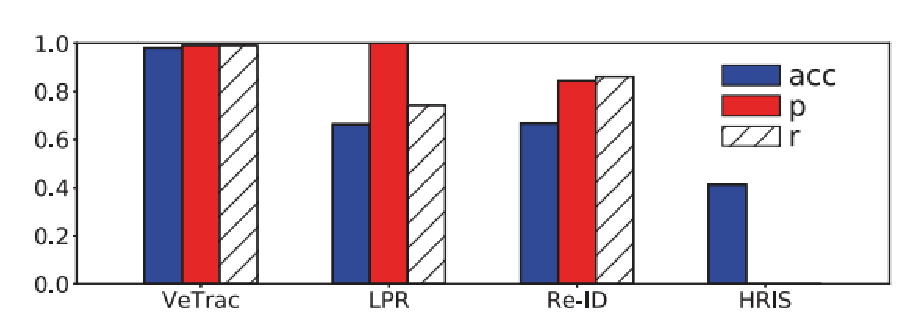
\includegraphics[width=0.9\linewidth]{figures/performance-comparison.eps}
  \caption{Performance comparison in express way \cite{tong2021large}}
  \label{fig:performance-comparison}
  %\vspace{-5mm}
\end{figure}

\begin{figure}
\centering
  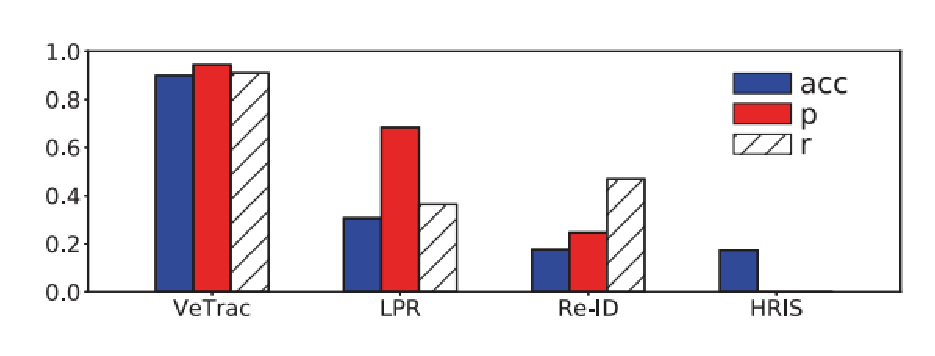
\includegraphics[width=0.9\linewidth]{figures/performance-comparison-urban.eps}
  \caption{Performance comparison inside city \cite{tong2021large}}
  \label{fig:performance-comparison-city}
  %\vspace{-5mm}
\end{figure}

Comparing the performance of VeTrac with the state-of-the-art networks for the blue ground-truth bus route in the city, depicted in \Cref{fig:bus-route-reconsturction-comparison}(a), the output is shown in \Cref{fig:bus-route-reconsturction-comparison}(b).
It is crystal clear that VeTrac reconstructed the correct track of the bus route with almost 100\% accuracy, while the routes generated in \ac{lpr}, \ac{re-id}, and \ac{hris} have lots of deficiencies.

\begin{figure*}
\centering
  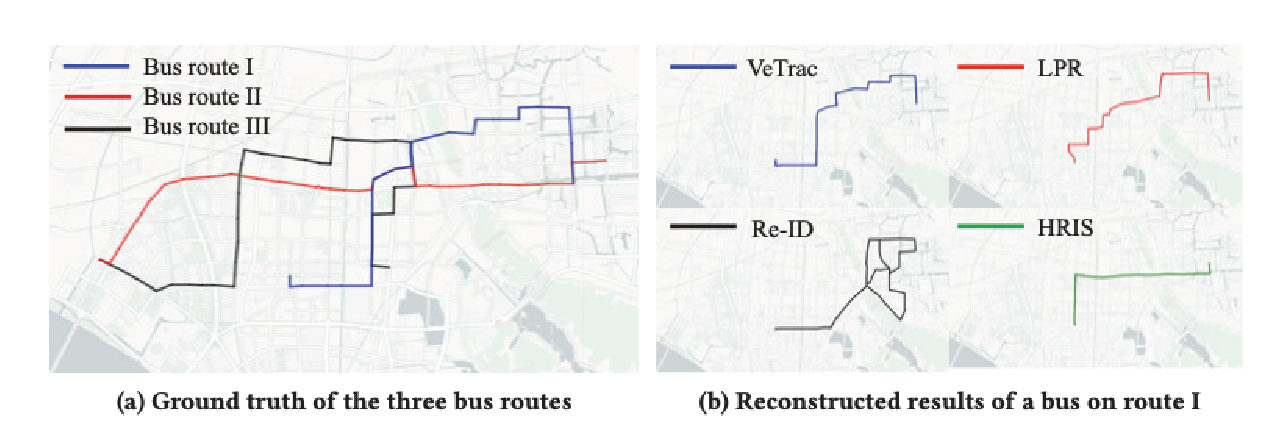
\includegraphics[width=0.9\linewidth]{figures/bus-route-reconstruction-comparison.eps}
  \caption{Bus route reconstruction comparison \cite{tong2021large}}
  \label{fig:bus-route-reconsturction-comparison}
  %\vspace{-5mm}
\end{figure*}

\section{Conclusions}
\label{sec:conclusions}

This study presented a vehicle trajectory reconstruction system that reconstructs the trajectories of generic traffics using widely deployed traffic cameras as a sensing network.
Large-scale studies with city-wide camera sensing data indicate that VeTrac has great accuracy and efficiency.
It is believed that VeTrac design gives insights that can be applied to various types of mobility studies.


\bibliographystyle{IEEEtran}
\bibliography{refs_LSVTR}

% \input{9. Appendices.tex}
\end{document} 